% 图 6.13 自旋链上的自旋波：(a) 透视——各进动盘上自旋方位角逐点推进 (b) 俯视——整排转过 360 度
\documentclass[tikz,border=5pt]{standalone}
\usetikzlibrary{arrows.meta}
\usepackage{amsmath}
\usepackage{bm}
\usepackage{fontspec}
\setmainfont{Times New Roman}
\begin{document}
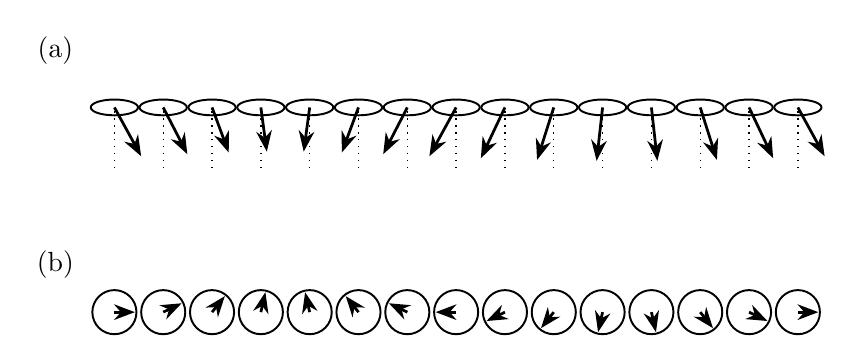
\begin{tikzpicture}[line width=0.8pt,>=Stealth]
\def\dx{0.62}
\def\step{25.7143} % 360/14: full turn across the row
% ================= (a) perspective view =================
\node at (-0.75,0.72) {(a)};
\foreach \n in {0,...,14}{
  \pgfmathsetmacro\x{\n*\dx}
  \pgfmathsetmacro\ph{\n*\step}
  % dotted cone axis
  \draw[dotted,line width=0.5pt] (\x,-0.05) -- (\x,-0.78);
  % precession ellipse
  \draw[line width=0.7pt] (\x,0) ellipse (0.30 and 0.10);
  % spin arrow: fixed polar angle, azimuth advancing site by site
  \draw[->,line width=1pt] (\x,0) --
    ({\x+0.34*cos(\ph)},{0.06*sin(\ph)-0.62});
}
% ================= (b) top view =================
\begin{scope}[shift={(0,-2.6)}]
\node at (-0.75,0.6) {(b)};
\foreach \n in {0,...,14}{
  \pgfmathsetmacro\x{\n*\dx}
  \pgfmathsetmacro\ph{\n*\step}
  \draw[line width=0.7pt] (\x,0) circle (0.28);
  \draw[->,line width=1pt] (\x,0) -- ({\x+0.26*cos(\ph)},{0.26*sin(\ph)});
}
\end{scope}
\end{tikzpicture}
\end{document}
